\documentclass{acm_proc_article-sp}
\usepackage{wrapfig}
\usepackage{graphicx}
\usepackage{caption}
\usepackage{subcaption}
\usepackage{tikz, alex, url, mu}
\usetikzlibrary{arrows,shapes,snakes,automata,backgrounds,petri}
\tikzset{>=stealth}

\title{Dynamic Cache Partitioning Based on Software Hints}

\author{Grant \and Jinilang}

\begin{document}
\maketitle

\begin{abstract}

Shared last-level cache has became the bottleneck of scalability in 
chip-multi-processors (CMPs) as one application's accesses to shared 
cache suffer from interferences caused by other cores' accesses. Cache 
partitioning has been proposed to partition shared cache among cores or
applications to alleviate interferences in shared cache. Existing cache
partitioning techniques assumes no prior knowledge is known about the 
applications before they starts running and thus may start with a terriable
initial partitioning. However, application developers, compilers or operating
systems may be able to provide software hints about the application's cache
usage beforehand. In our work, we studied what kinds of software hints might be 
useful and how they might be used assuming those hints could be generated. We
designed and implemented a system that uses software hints for cache 
parititioning. Evaluations showed that software-hinted cache paritioning indeed
improves shared cache performance in terms of total number of misses. Our work
provides the first step for future works on software-hinted cache paritioning.

\end{abstract}

\section{Introduction}

In traditional chip-multi-processors (CMPs), the last-level cache is 
shared among all cores and LRU is usually used as the replacement policy. Shared
last-level cache is long konwn to suffer from interference among cores. The 
LRU policy implicitly partitions the shared cache among cores based on their 
requests for cache resources. The resulted cache partitioning among cores is
unlikly to be optimal in terms of the total number of cache misses. This is 
because the marginal benefit gained from increasing cache space differ across 
cores. Limited cache resources should allocated to applications that may get
more marginal benefits from them.

Application developers might be able to predict their applications' cache usage 
and thus request an optimal amoumt of shared cache for his application. For 
example, the application developer might know that his application is a 
streaming application. In that case, although the application demands a large 
amount of cache, the marginal benefits the application gains from the additional
cache space is small. Thus he requests a small amount of cache according the 
application's working set size. So application programmers may provide hints for
requesting shared cache space.

Compiler might be able to analyze the program at compile time and predict the 
application's working set size and thus make request accordingly. The operating
sytem might be able to analyze the application's live trace and utilize more 
sophisticated algorithms to predict its working set size that what can be done
in hardware. Thus the operating system might as well provide hints for 
requesting shared cache space.

We understand that generating those hints might be a hard problem itself. 
However, as a logical first step, we'd like to know whether those hints would 
be helpful assuming idea hints can be generated. Therefore, in this project, we 
performed a limit study and designed a cache partitioning mechanism based on 
software hints to investigate how software hints may be utilized in cache 
partitioning to minimize cache misses. We believe our work can serve as the 
foundation of future works that intend to investigate cache partitioning based
on software hints.

\section{Background and Related Works}

Serveral cache partitioning mechanisms have been proposed by previous works 
to minimize cache misses in shared cache.
\cite{Qureshi:2006:UCP:1194816.1194855} proposed a utility-based cache 
partitioning strategy. In their approach, each core is associated with a utility
monitor (UMON). UMON has a tag directory which caches a tag per set per way. 
In order to reduce hardware overhead, UMON may cache only one tag for the same 
cache way in all sets. By using UMON, a cache miss line can be obtained, which 
depicts the relationship between number of cache misss and the number of ways 
assigned to this core. By greedily assigning each cache way to the core where 
the cache utility can be maximized (reducing most cache misses), this approach
partitions the cache to maximize utility (minimize cache misses). This is called
look ahead algorithm.

\cite{Qureshi:2006:CMC:1150019.1136501} pointed out that cache misses are not 
equivalently expensive. Parallel misses are much cheaper than isolated misses 
because they can be served in parallel. Instead of minimizing the number of 
cache misses, a better cache partitioning strategy might be minimizing MLP-based
cache cost. This strategy was explored by \cite{conf/IEEEpact/MoretoCRV07} which
demonstrated MLP-aware cache partitioning indeed achieves better performance.
Recently, \cite{conf/IEEEpact/BeckmannS13} studied partitioning fully-associated
cache to data and it reduced the cost of look-ahead algorithm by peek-ahead 
algorithm.

All previous works predict future cache usage based on previous cache miss 
curve. This works if the cache usage pattern remains similar across different 
phases of the program. When the memory usage pattern of the program changes 
across phases, the prediction might be inaccurate. In our project, we'd like to
further improve cache partitioning based on program hints for future memory 
usage given by users, OS, or compiler.

\cite{Ipek:2008:SMC:1381306.1382172} describes a novel memory controller design
 which would use adaptive 
scheduling based on machine learning. Using reinforcement learning, their 
scheduler would optimize scheduling on the fly. Controller-state action pairs 
are assigned reward values, and when commands are issued, the controller tries 
to choose the command with the greatest long term value. A learning controller 
brings about some great benefits to program performance. Primary amongst these 
is that the controller optimize for bus bandwidth, and does so on the fly. Many 
scheduling algorithms attempt provide the best bandwidth in the general case, 
though there often weak spots in their approaches which reduce memory 
throughput. By learning and being adaptable, the authors’ scheme fights this 
weakness. In addition, the rewards system takes the core where the memory 
request originated from, allowing the scheme to fight against starvation as 
well. However the capabilities of the scheduling system are limited. While in 
theory, the machine learning algorithm they chose should be able to take into 
account infinitely many states and inputs, hardware and computation time hampers
 the scheduling optimization possibilities. While the authors optimized their 
algorithm for the resources they had available, there are various scenarios 
which they were not able to account for due to hardware limitations, creating 
weak spots in their system.

\cite{10.1109/MM.2008.48} proposes a thread scheduling scheme to minimize LLC 
con-tention based on 
architectural observations made by the OS at run- time. While the paper does 
not discuss the modification of architectural features, it demonstrates how the 
OS can interface with the architecture to find optimize system behavior. In this
 particular instance, by leveraging features of the chosen architecture, the 
authors were able to track cache hit/miss ratios as well as absolute counts of 
hits and misses on caches in the system. Using these metrics, threads running in
 the system were assigned weights which corresponded to their cache usage. 
Threads were then scheduled on the cores in such a way that these weights were 
spread as evenly as possible across shared caches. The benefits to this approach
 are easily tangible. Scheduling threads in this way ensures that memory 
intensive processes are given an appropriate amount of resources rather than 
being forced to share an unnecessary and counter productive portion of cache. 
The feature we are proposing could possibly extend this scheme by allowing the 
OS to interface with shared caches to get better partitioning.

Previous approaches assume nothing is known about the application in prior and 
thus can only partition the shared fairly among cores. Since those approaches 
rely on analyzing runtime statistics and dynamically adjusting cache partition,
it may take too long for them to converge to an optimal partition. Also, since 
they rely on analyzing runtime application behavior, those approaches demand 
higher hardware cost and introduce runtime overhead. In contrast, our approach
introduce lower hardware complexity and lower runtime overhead.

\section{Proposed Technique}

An application may have multiple phases and it may have different needs for 
cache in different phases. Our proposed framework would allow the application to issue 
cache requests anytime during the course of the program. The request specifies 
the working set size of the application in the upcoming phase. The shared cache
takes into account the requests from all cores and partition the shared cache
propotionally according to their working set size. We refer to this as 
\emph{working-set-size-based partitioning}. Our basic technique is visualized 
in Figure~\ref{fig:hinted_partition}

However, the above partitioning approach has its limitations. While it allows the
cache to take into account working set sizes of applications, it is completely ignorant
of an application's cache sensitivity. With the basic technique, while two applications
may have similar working sets, one program may have much more sparse cache accesses.
The ideal approach would be able to take into account cache access frequency as well. 
Thus, besides the basic partitiong approoach above, we also propose a more 
sophisticated partitioning strategy. Instead of providing a single number of 
working set size, the software hint may provide a cache miss curve at each 
phase. This miss curve would consist of the MPKI over a range of cache sizes. 
Knowing these cache miss curves would allow the shared cache to analyze the 
marginal benefits of allocating shared cache space to each core and thus achieve
the optimal partition that miminizes cache miss rate for the entire system. We refer to this as 
\emph{cache-miss-curve-based partitioning}.

Programs consist of functions. In our approach, application phases are marked by
function boundaries. Thus reqeusts for shared cache are issued every time the 
application enters a function.

\begin{figure}[th!]
  \label{fig:hinted_partition}
  \centering
  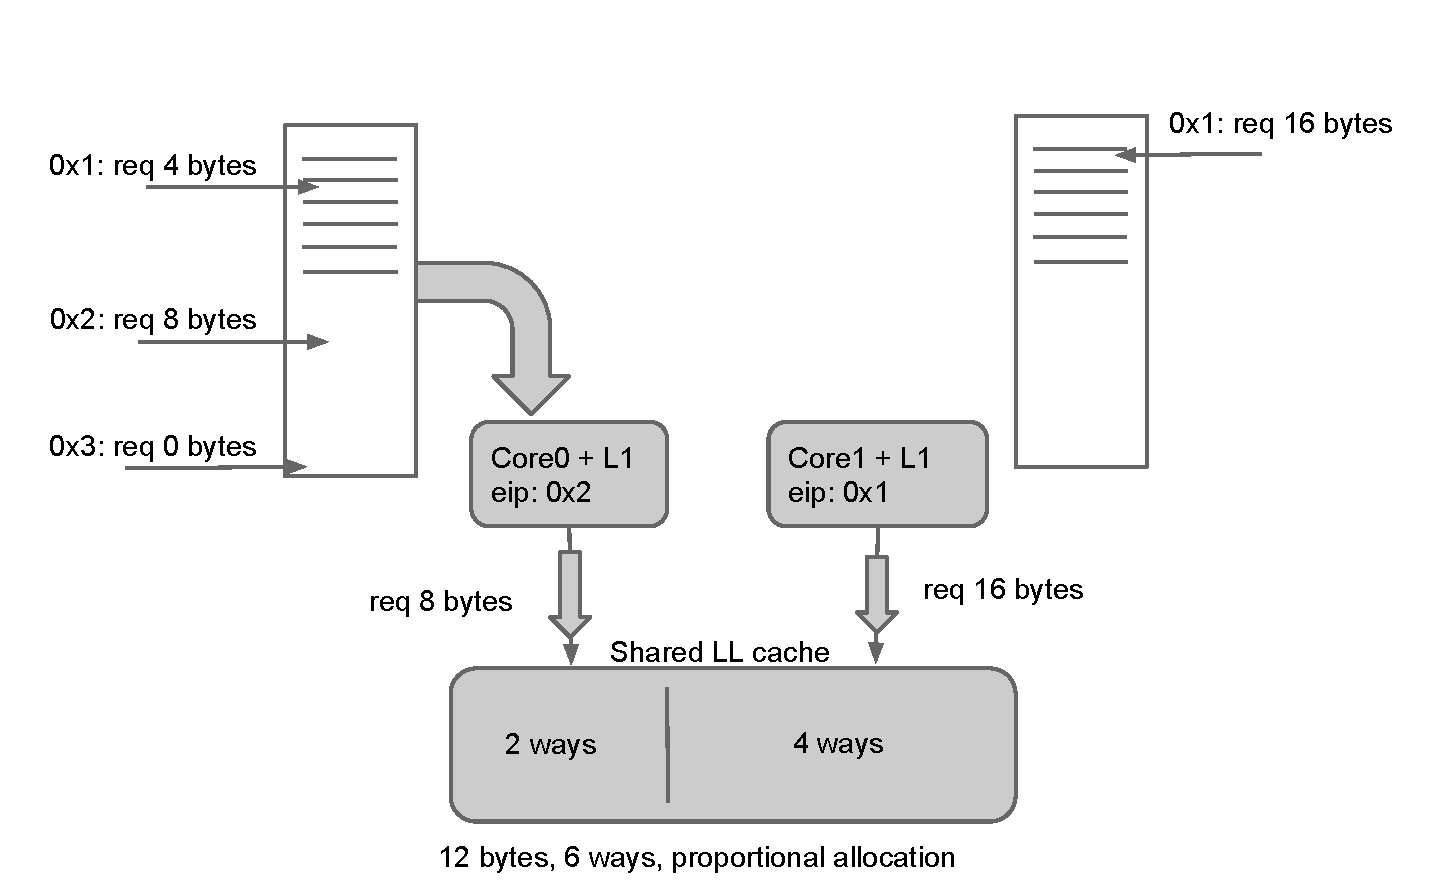
\includegraphics[width=.5\textwidth]{figs/hinted_partition.pdf}
  \caption{\small Visual illustration of shared cache partitioning based on software 
    requests of working set sizes. Firstly, application 1 issues its request 
    of 4 bytes and application 2 issues its request of 16 bytes. Core0 and Core1 
  forwards the requests to the shared cache. The shared cache then partitions 
  ways propotional to the working set sizes of each application. Thus 2 ways are 
  allocated for core0 and 4 ways are allocated for core1. When application 1 issues
  a new request for shared cache, the shared cache re-partitions ways 
  accordingly.}
\end{figure}



\section{Implementation and Evaluation Methology}

The propsed technique requires our framework to take in cache request any time 
and adjust cache partitioning accoridngly. However, this was too complicated to
implement. Due to limitation of time, we resorted to a simplified 
implementation. Instead of letting the application issue cache requests at 
phase changes, we only let applications issue cache requests when the program
starts. The shared cache is partitioned according to the requests and the 
partitioning is used for the entire course of the program.

Our technique is implemented on a simulator Multi2Sim \cite{multi2sim}, 
which is used for evaluation. We used Mediabench as our benchmarks 
\cite{mediabench}.

In order to evaluate our proposed partitioning strategy, we need to predict the 
working set size and the cache miss curve of each function. To learn the cache 
miss curve of each function, we used a tool called Cachegrind \cite{cachegrind}
which simulates a cache of user-specified configuration and reports statistics 
about the program running with the give cache setting. It may also report 
statistics of each function of the program. Thus, by varying the size of shared 
cache, we obtained the cache miss curve of the entire program as well as that of
 each function.

In order to evaluate the \emph{working-set-size-based partitioning}, we need to 
know the working set size of each applications. We obtained that from each 
application's cache miss curve. We show a few applications' miss curves in Figure~\ref{fig:miss-curve}. 
We consider the working set size to be the point where the cache miss rate stops dropping rapidly as the cache size increases. In other words, it's where the slope of the cache miss curve decreases 
significantly. For some applications, such as those shown in 
Figure~\ref{fig:epic-decode} and Figure~\ref{fig:epic-encode}, this point is 
obvious. For some other applications, such as those shown in 
Figure~\ref{fig:jpeg-decode} and Figure~\ref{fig:jpeg-encode}, it's not obvious
where the marginal benefit of increasing cache size drops. In such cases, we 
might make a bad decision in choosng working set sizes. Some of the
effects of choosing a bad working set can be seen in Section~\ref{sec:results}.

The \emph{cache-miss-curve-based partitioning} was evaluated in a similar way.
Due to the relatively static nature of our simulator implementation, no reimplementation
was required. Working set sizes which summed to the size of the cache, thus
corresponding directly to the number of ways to be assigned to a core's partition.
To obtain the optimal partition for this mechanism, the two miss curves were overlaid
in opposite directions. The reason for this is due to the fact that partitioning acts like a sliding scale
between applications. Sliding one way will cause fewer misses for one application, but more for the
other. By overlaying the curves in this manner, their point of intersection will indicate the optimal partitioning
between the two applications. At the point where the curves meet, the marginal utility lost by each application
is equal. Here, marginal utility is measured in cache misses per instruction. The start and end point for each miss curve corresponded directly to the size of the cache. For our simulations, the miss curves were cut off at a size of 3584,
as a single collection of ways across the sets of the cache sums to 512 bytes, and no
application can take all ways, or have none. For some application pairs, the miss curves intersected at a simulatable
size point, while for others the intersection fell between points. In these cases, the nearest size point was chosen. 
If we had been able to simulate a larger cache, we could have increased the granularity of the ways. However,
this was not the case and thus must be addressed in a future work.


\section{Results and Analyses}

The initial step of our project was to evaluate the performance of our working set based implementation. As can be seen in Figure~\ref{fig:hinted_partition}, over our relatively small sample size, the results show an improvement. However in the case of running Epic Encode and Epic Decode together, the working set selection used in the simulation caused a 
massive degradation in performance. This revealed one of the dangers with simple working set partitioning. While it is simple for a developer to ascertain the working set of his program, it is impossible for the cache to weight two similar working sets against each other. As can be seen from the 

\begin{figure}
        \centering
        \begin{subfigure}[b]{0.25\textwidth}
          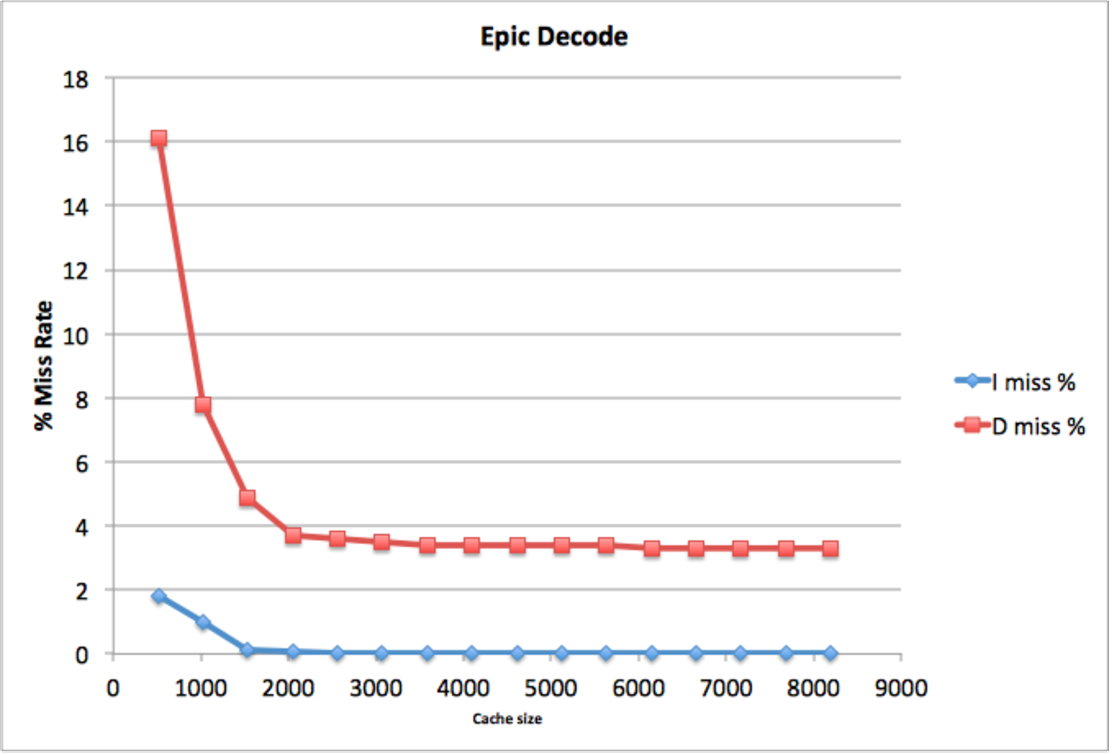
\includegraphics[width=\textwidth]{figs/epic-decode-miss-curve.pdf}
          \caption{Epic-decode}
          \label{fig:epic-decode}
        \end{subfigure}%
        %\quad
        \begin{subfigure}[b]{0.25\textwidth}
          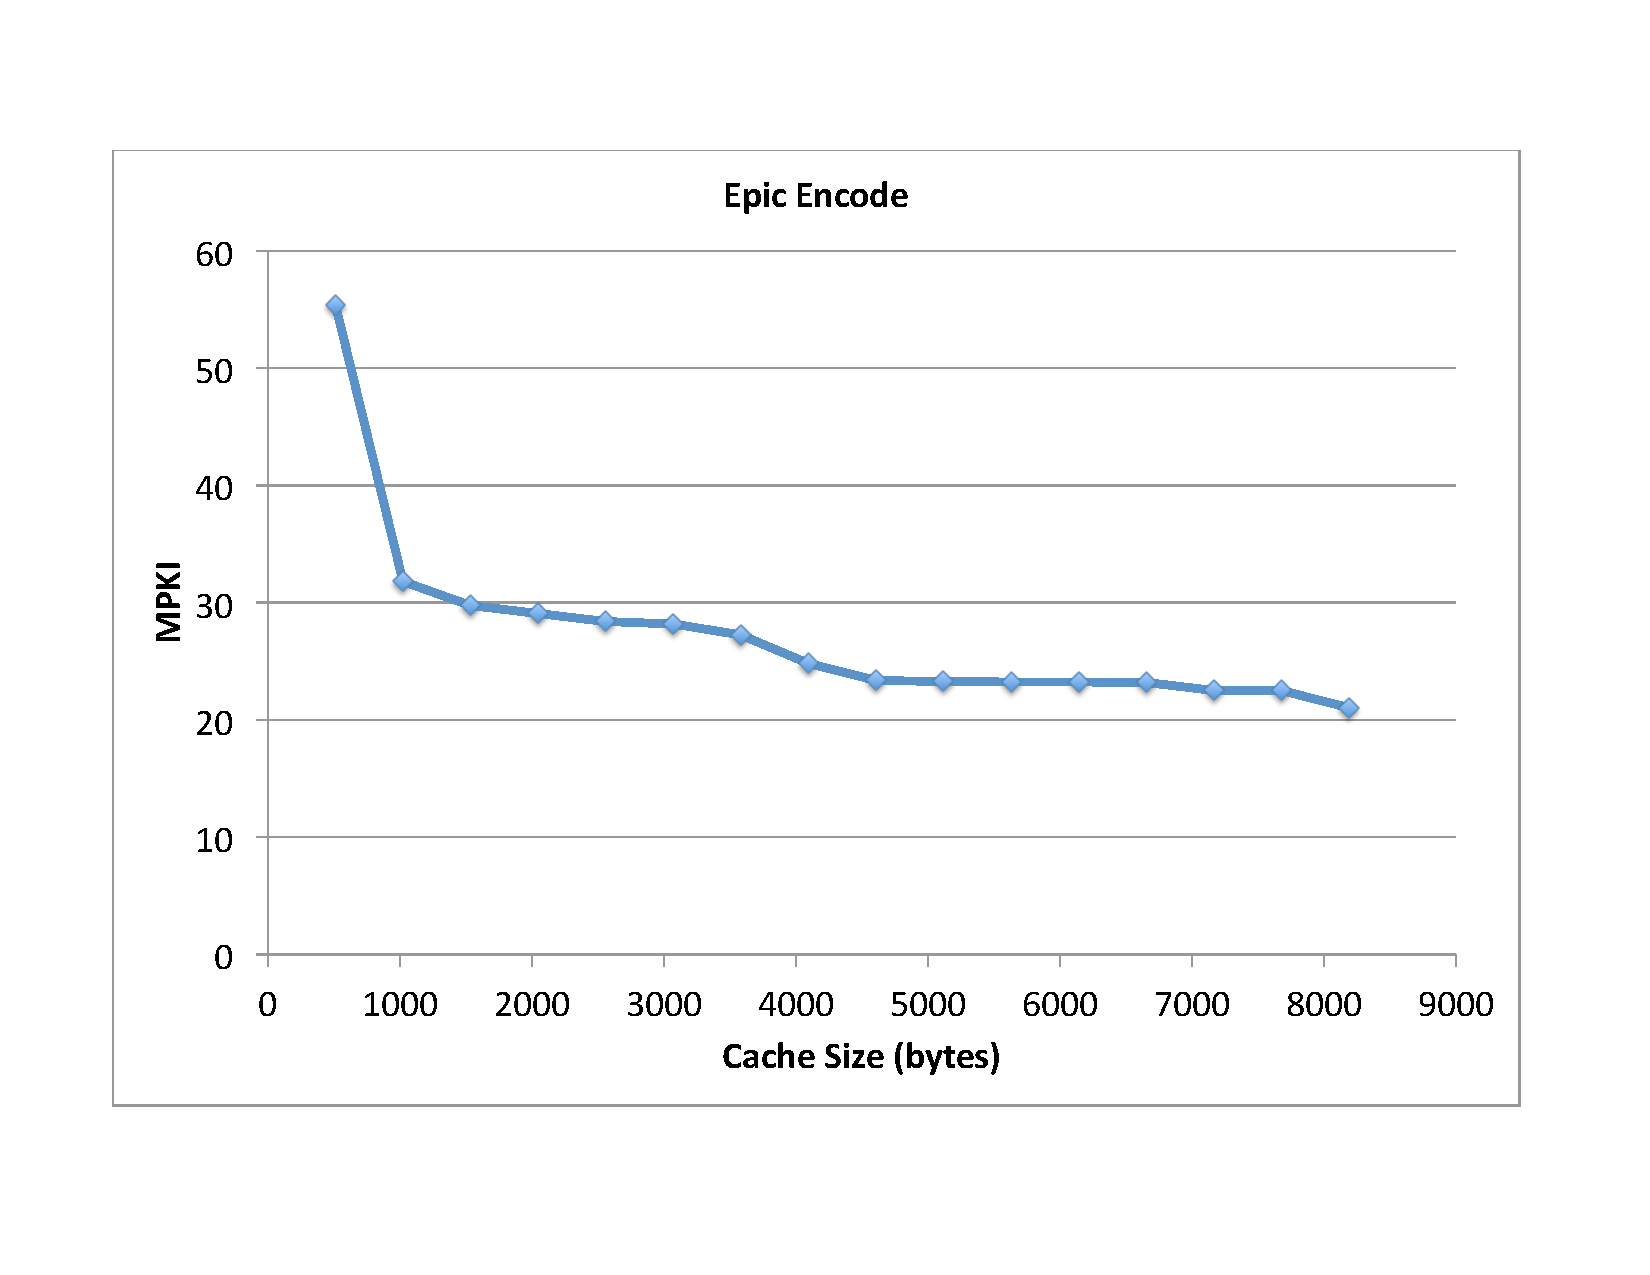
\includegraphics[width=\textwidth]{figs/epic-encode-miss-curve.pdf}
          \caption{Epic-encode}
          \label{fig:epic-encode}
        \end{subfigure}

        \begin{subfigure}[b]{0.25\textwidth}
          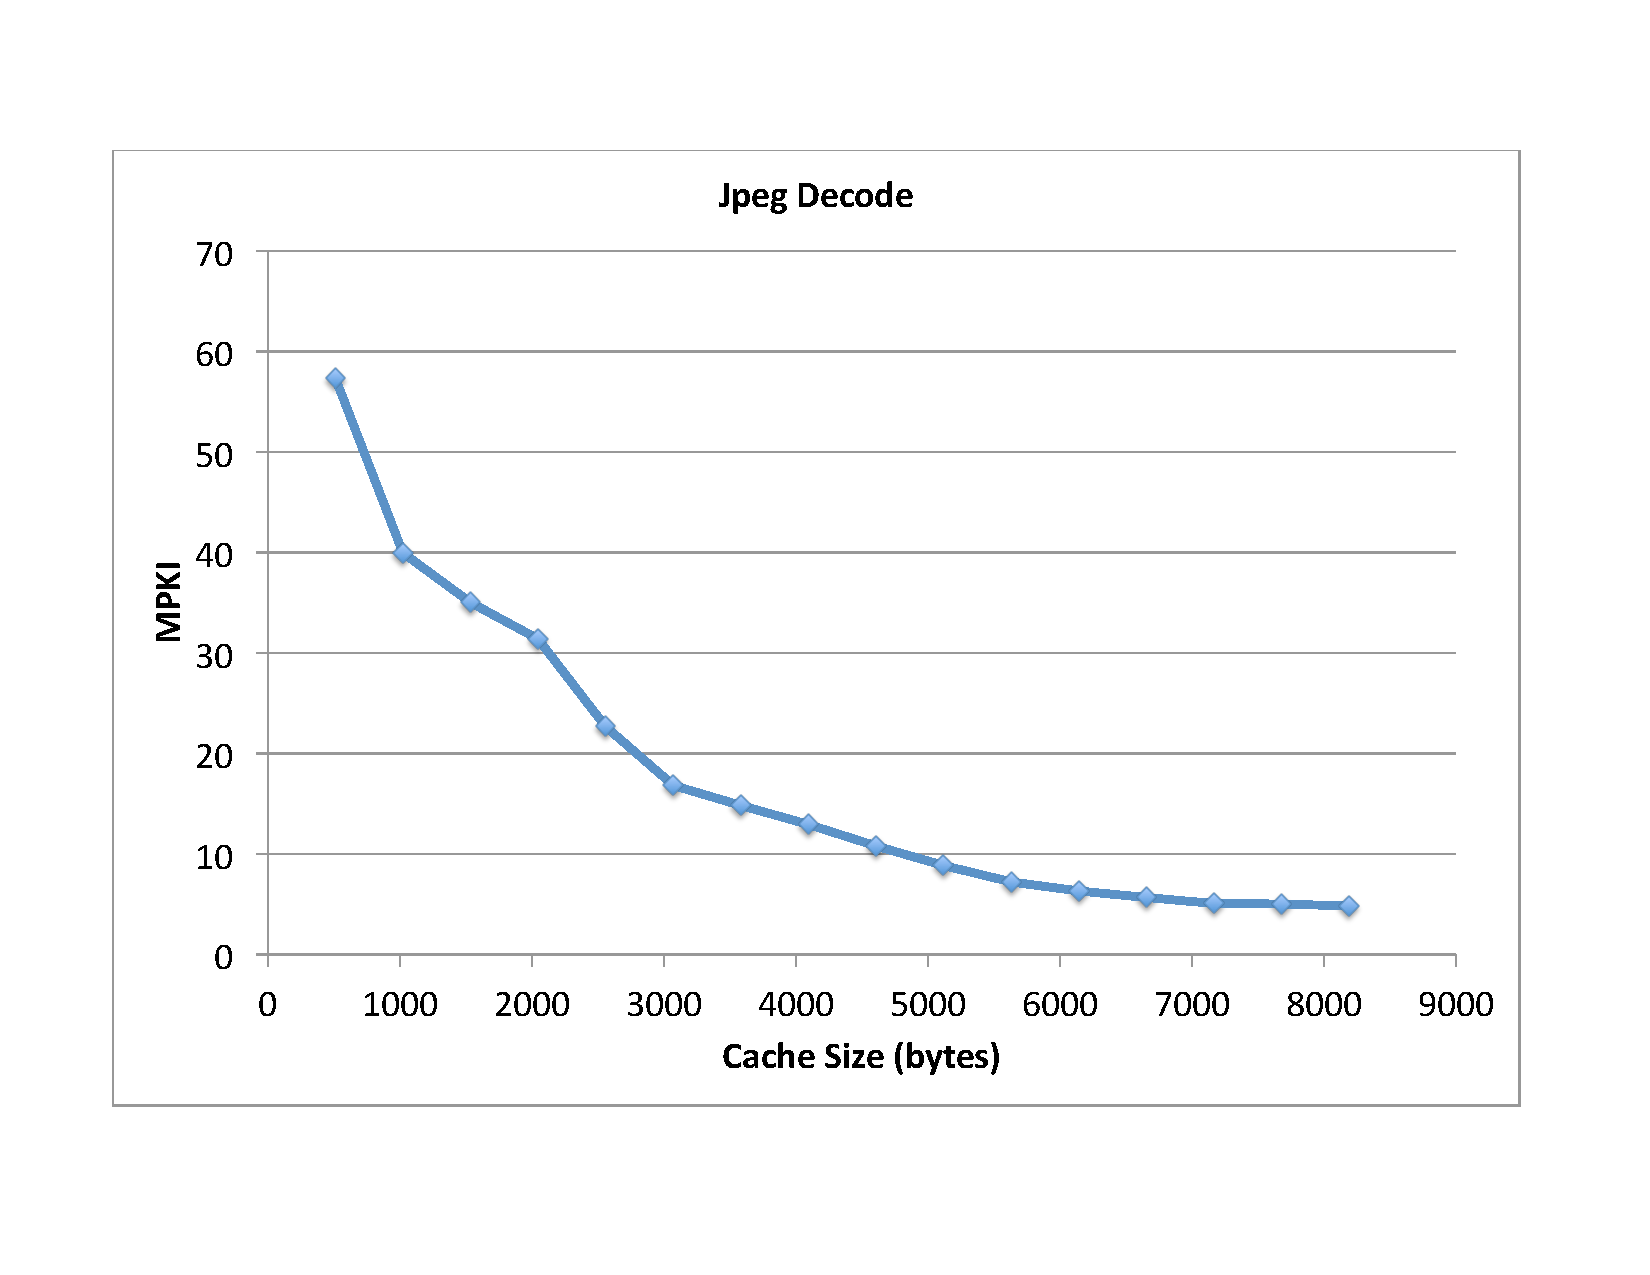
\includegraphics[width=\textwidth]{figs/jpeg-decode-miss-curve.pdf}
          \caption{Jpeg-decode}
          \label{fig:jpeg-decode}
        \end{subfigure}%
        %\quad
        \begin{subfigure}[b]{0.25\textwidth}
          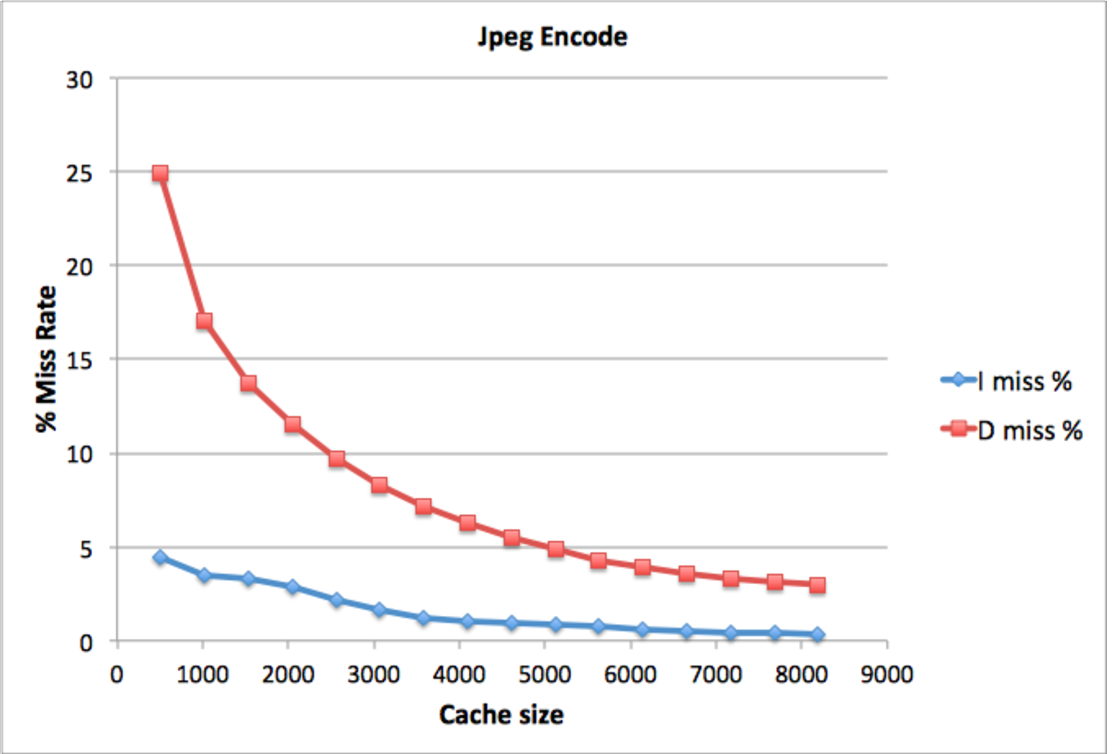
\includegraphics[width=\textwidth]{figs/jpeg-encode-miss-curve.pdf}
          \caption{Jpeg-encode}
          \label{fig:jpeg-encode}
        \end{subfigure}
       \caption{Example applications' miss curves}
       \label{fig:miss-curve}
\end{figure}

\section{Results and Analysis}
\label{sec:results}

\subsection{Working-Set-Size-Based Partitioning}

Firstly, we show experiment results of working-set-size-based partitioning in 
Figure~

\begin{figure}
  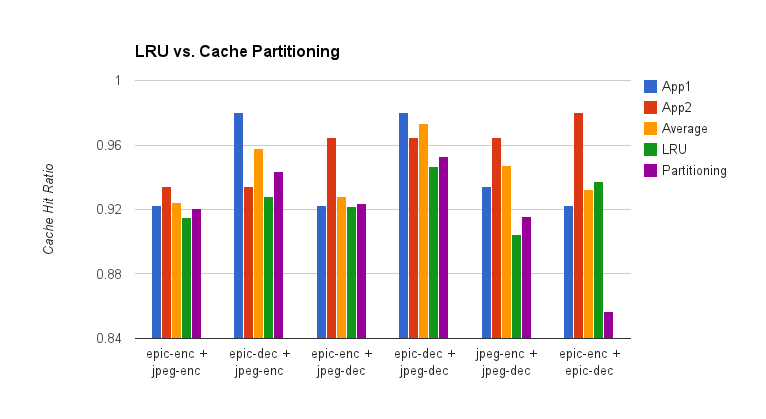
\includegraphics[width=0.5\textwidth]{figs/work_set_size_hit_ratio.png}
\end{figure}

\section{Lessons Learned, Shortcomings, and Future Work}
 
While the investigation yielded interesting results with potential, many shortcomings prevented it from being thorough and definitively conclusive. First and foremost among these shortcomings was lack of access the SPEC2006 benchmark workloads. This shaped our non-standard simulation set up. As a substitute, we used Mediabench I and associated sample workloads, which only began to display poor locality at cache sizes of 4 kb. Though we were able to modify our simulator layout to account for this, the resulting simulation results may not relate well to the most current benchmarks and workloads.
 
Beyond the shortcomings of the benchmarks we had used, and the resulting effects on the simulations we ran, there were many lacking points in our custom simulator implementation. We were able to implement cache partitioning over the entire run of the program, which was a good proof of concept. However, in our original plan we stated that we would investigate the potential of software hints at phase changes in the program via function profiling. However, for the benchmarks we used, we were unable to reverse engineer the call graphs for our test programs from the provided binaries. Though cachegrind was able to count cache misses per function, this data was useless without knowledge of these functions’ placement in the program.
 
In addition, in our custom simulator did not implement partitioning via Utility Monitoring. This was meant to be the prime point of comparison for our study, as our software hints implementation essentially places the burden of utility monitoring onto the developer.  However, we were unable to implement utility monitoring in our simulator and thus we were unable to study it. On the other hand, considering the fact that our partitioning solution was largely incomplete, it likely would not have had a strong chance of competing against a UMON partitioning solution. Our tested implementation was essentially static, whereas UMON allocates ways dynamically.
 
The work we have done is essentially a proof of concept, which we believe shows that software hints have great potential for future cache partitioning implementations. Logical future steps, as outlined, would be to test against contemporary benchmarks and to use a simulator setup commensurate with modern architectures, implement a dynamic partitioning solution and make a comparison against partitioning via Utility Monitoring.

\section{Conclusion}

We introduced a mechanism for allowing developers to provide software hints to shared caches. Our technique amounts to allowing developers to make allocation requests into a shared last level cache. This allows the cache to intelligently allocate cache-ways to applications running on different processor cores such that cache space is maximally used by the system. Although the original implemented solution simply consisted of requiring developers to indicate working set size, we created a more advanced implementation which took into account cache sensitivity as well as working set size. The final experimental implementation compared running applications’ marginal utility curves to determine the optimal way partitioning for the system. This implementation shows improvement over naïve LRU replacement as well as simple static partitioning methods. The next logical step in our implementation would be to implement capability for dynamic requests. Further, we wish to compare this implementation to utility monitoring based partitioning solutions, or even augment our final solution with utility monitoring to determine the greatest point to which cache partitioning can be maximized.


\bibliography{ref}
\bibliographystyle{plain}

\end{document}
